\documentclass{article}

\usepackage[utf8]{inputenc}
\usepackage[T1]{fontenc}
\usepackage[francais]{babel}
\usepackage{url}
\usepackage{color}
\usepackage{verbatim}
\usepackage{amsmath,amssymb,amsfonts}
\usepackage{graphicx}
\usepackage[french]{algorithm2e}
\usepackage{geometry}
\usepackage{caption}
\captionsetup[figure]{slc=on}
\usepackage{enumitem}
\usepackage{listings}
\usepackage{listingsutf8}
\frenchbsetup{StandardLists=true}
\lstset{
	breaklines=true, 
	showspaces=false, 
	keepspaces=true, 
	numbers=left,
	frame=shadowbox, 
	keywordstyle=\color{blue},
	basicstyle=\ttfamily\small,
	commentstyle=\color{green}
}
\geometry{hmargin=2.5cm, vmargin=2.5cm}

\title{\textbf{TP09 : Projet de Synthèse d'Images}\\Génération de terrain aléatoire}
\author{Line \bsc{POUVARET}, Mickaël \bsc{TURNEL}, Antoine \bsc{THEBAUD}}
\date{2015-2016}

\begin{document}
\maketitle
\section{Présentation de notre projet}

Nous avons réalisé un programme de génération de terrain qui utilise un bruit de Perlin pour créer un champ de hauteur.\\

Voici l'ordre détaillé des étapes que nous réalisons.

\subsection{Première passe : génération du bruit}
Elle consiste à générer le bruit grâce à un shader approprié (noise.vert, noise.frag).

On envoie au vertex shader également le vecteur de mouvement qui va nous permettre de modifier la map de bruit générée en fonction de celui-ci.

Le bruit ainsi généré est produit dans une texture de la taille de la grille du terrain que l'on dessine dans un fbo.\\

\subsection{Deuxième passe : normales}

Celle-ci sert à générer la map des normales des sommets en utilisant d'autres shaders (normal.vert, normal.frag).

Le fragment shader se sert bien évidemment de la map de hauteur générée précédemment.

Encore une fois, elle est générée dans une texture dessinée dans le même fbo.\\

\subsection{Troisième passe : shadow map}
Après cela, nous avons une passe à part pour générer la shadow map de notre rendu dessinée dans un autre fbo (shadow-map.vert, shadow-map.frag).

Dans le vertex shader, nous mettons à jour la position des sommets selon l'espace de lumière (matrice de modèle-vue-projection) et on ne fait rien dans le fragment shader.

Nous utilisons des soft shadows avec la Loi de Poisson pour générer nos ombres.\\

\subsection{Quatrième passe : rendu}
Enfin, on rend notre scène en réalisant un displacement mapping selon le champ de hauteur généré. (rendering.vert)

\subsection{Cinquième passe : post-process}

On ajoute un Phong shading dans le fragment shader pour la lumière (en utilisant la normal map) ainsi que nos ombres projetées grâce à la shadowmap. (rendering.frag)\\

Toujours dans le fragment shader du rendu, on ajoute un effet de brouillard blanc sur la scène en fonction de la profondeur par rapport à la position de la caméra.

Et pour finir, nous utilisons des textures 2D qui nous permettent de déterminer la couleur d'un fragment selon la hauteur.

\section{Fonctionnalités du programme}

Les paramètres du bruit sont les suivants :
\begin{itemize}
	\item amplitude : 50.0
	\item fréquence : 2.0
	\item persistance : 0.4
	\item nombres d'octaves : 10.0
\end{itemize}

Il y a la possibilité de "naviguer" dans le terrain en appuyant sur la touche Z pour avancer et S pour reculer.

Le mouvement du terrain suit le mouvement de la camera si on laisse le clic gauche appuyé.\\

Il est également possible de "descendre" et "monter" le terrain sachant qu'il n'a qu'une limite en descente (au niveau de l'eau) avec les touches Q et D (Q pour descendre, D pour monter).\\

Le rendu de lumière, les ombres projetées et le brouillard peuvent être activées/désactivées individuellement.\\

Nous utilisons une texture 2D qui nous sert de colormap sur le terrain.

Chaque pixel de sommet recevra le pixel de la texture qui lui sera associé grâce à sa hauteur.\\

Il y a aussi la possibilité d'utiliser plusieurs textures individuelles qui seront appliquées selon la hauteur du sommet.\\

On peut aussi afficher les différentes map du programme à savoir :
\begin{itemize}
	\item la height map
	\item la shadow map 
	\item la normal map
\end{itemize}

Celles-ci changent bien évidemment lorsque l'on se déplace avec les touches Z et S.

\subsection{Description des raccourcis clavier}
\begin{itemize}
	\item Z : avancer
	\item S : reculer
	\item Q : descendre
	\item D : monter
	\item W : afficher/masquer la shadow map
	\item C : afficher/masquer la normal map
	\item X : afficher/masquer la height map
	\item L : activer/désactiver le rendu de lumière
	\item G : activer/désactiver les ombres
	\item B : activer/désactiver le brouillard
	\item F : afficher les fps
	\item T : changer de mode de texture (entre la texture 2D colormap et les textures individuelles)
	\item I : réinitialiser
\end{itemize}

\subsection{Description des raccourcis souris}
\begin{itemize}
	\item clic gauche enfoncé : permet de bouger l'angle de la caméra
	\item clic droit : permet de modifier la position de la source de la lumière
\end{itemize}

\section{Captures d'écran}

\subsection{Au lancement du programme}
Voici la capture d'écran obtenue au lancement du programme :
\begin{figure}[h]
	\center
	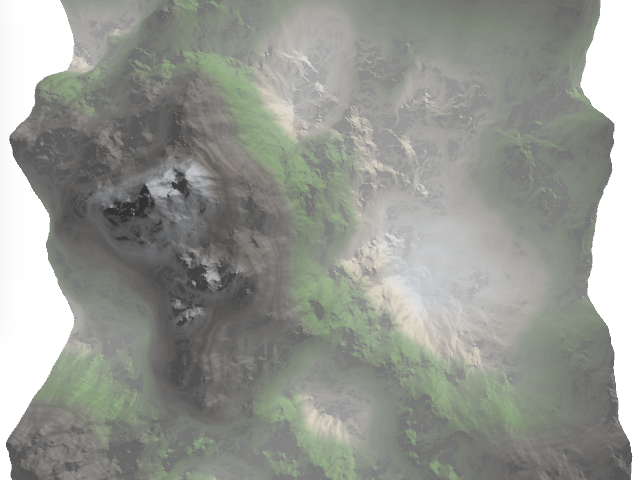
\includegraphics[scale=0.30]{screen0.png}
	\caption{Vue du terrain au lancement}
\end{figure}

La vue par défaut est par dessus le terrain.
\newpage
En laissant le clic gauche enfoncé et en faisant un mouvement vers le haut, on obtient cette vue :

\begin{figure}[h]
	\center
	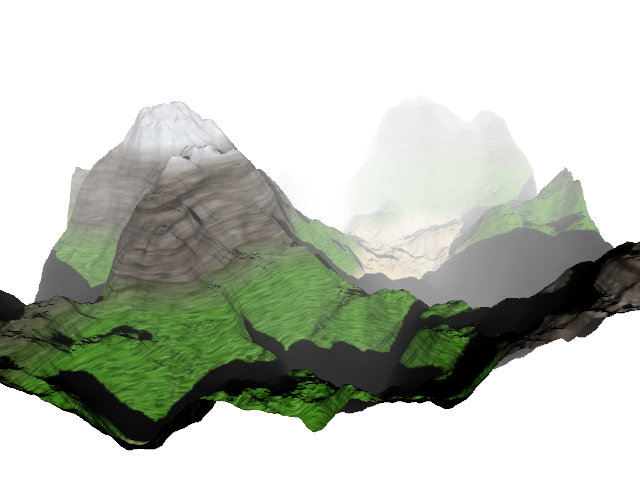
\includegraphics[scale=0.30]{screen1.png}
	\caption{Vue du terrain de face}
\end{figure}

\subsection{Activer/désactiver des post-process}

On observe que nous avons par défaut les ombres, la lumière et le brouillard.

Si l'on désactive le brouillard, on obtient cette vue :

\begin{figure}[h]
	\center
	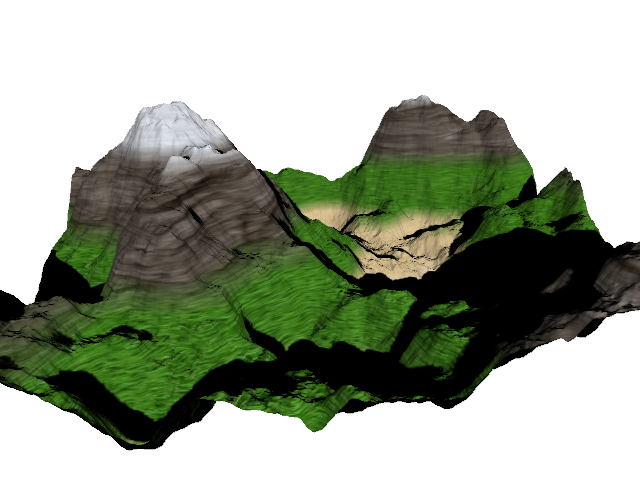
\includegraphics[scale=0.30]{screen2.png}
	\caption{Terrain sans brouillard}
\end{figure}
\newpage
Si l'on désactive uniquement les ombres, on obtient cette vue :

\begin{figure}[h]
	\center
	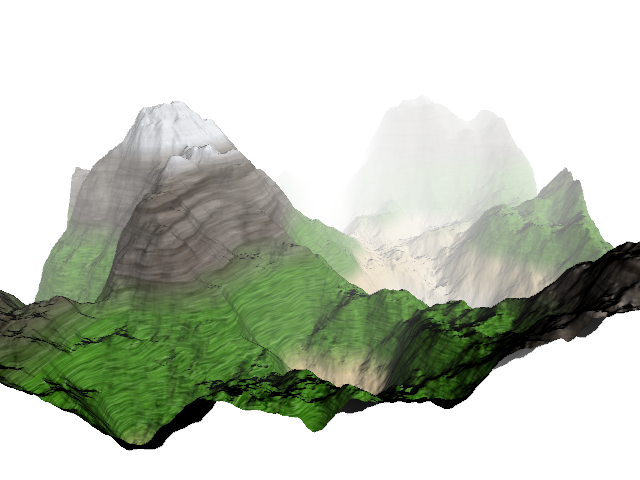
\includegraphics[scale=0.30]{screen3.png}
	\caption{Terrain sans ombres}
\end{figure}

Si l'on désactive uniquement la lumière, on obtient cette vue :

\begin{figure}[h]
	\center
	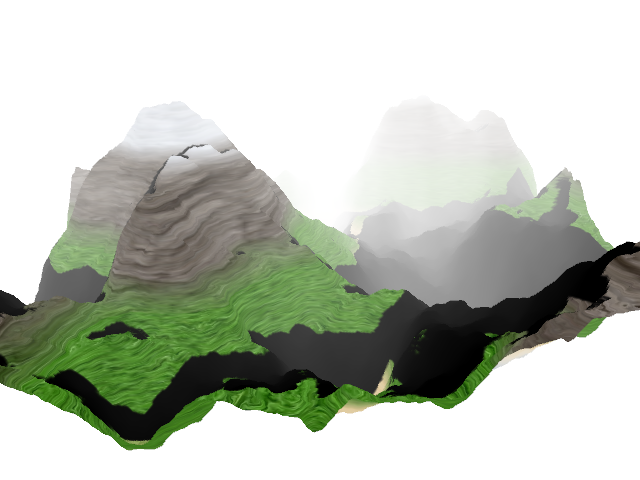
\includegraphics[scale=0.30]{screen4.png}
	\caption{Terrain sans lumière}
\end{figure}
\newpage
Et enfin, si on désactive les trois, on obtient cette vue (beaucoup moins agréable à regarder):
\begin{figure}[h]
	\center
	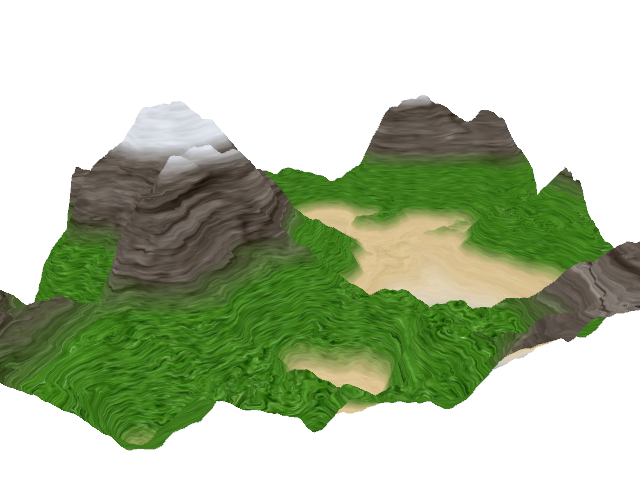
\includegraphics[scale=0.30]{screen5.png}
	\caption{Terrain sans ombres, brouillard, lumière}
\end{figure}

\subsection{Afficher/Masquer les map}
\subsubsection{La height map}

\begin{figure}[h]
	\center
	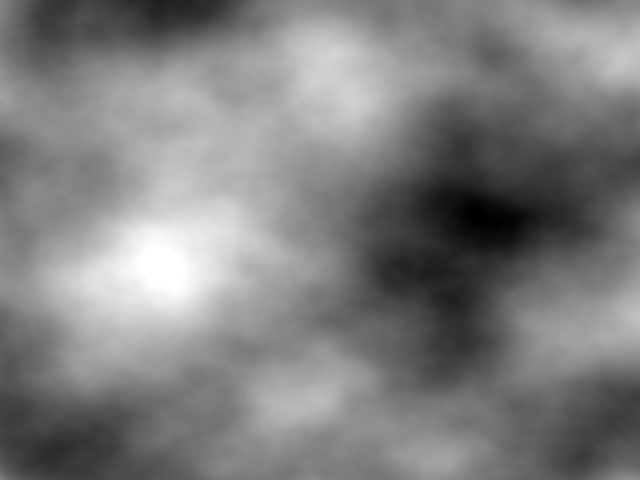
\includegraphics[scale=0.30]{screen7.png}
	\caption{height map}
\end{figure}
\newpage
\subsubsection{La normal map}

\begin{figure}[h]
	\center
	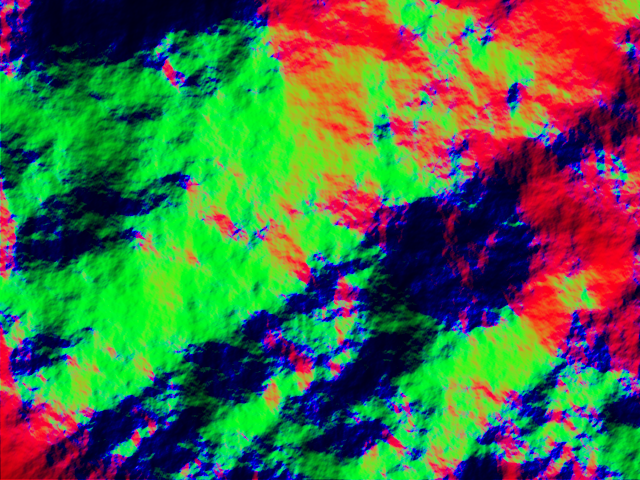
\includegraphics[scale=0.30]{screen8.png}
	\caption{normal map}
\end{figure}

\subsubsection{La shadow map}

\begin{figure}[h]
	\center
	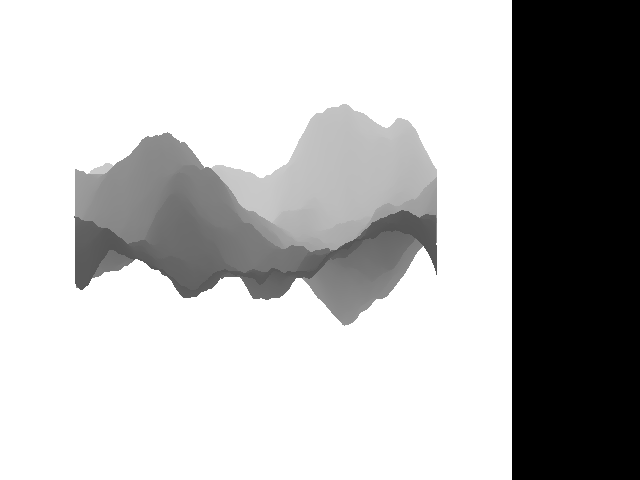
\includegraphics[scale=0.40]{screen6.png}
	\caption{shadow map}
\end{figure}
\newpage
\subsection{Changer le mode de texture}

Voici l'affichage d'une scène de notre terrain avec la texture 2D de type colormap :

\begin{figure}[h]
	\center
	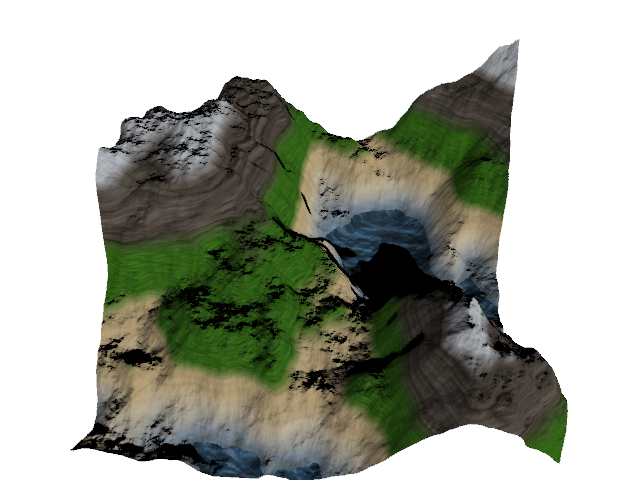
\includegraphics[scale=0.30]{screen9.png}
	\caption{Scène avec texture 2D colormap}
\end{figure}

Et voici l'affichage de la même scène avec les textures 2D individuelles :

\begin{figure}[h]
	\center
	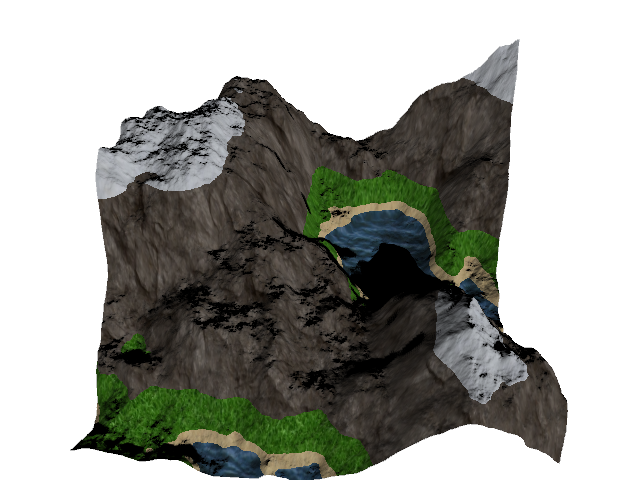
\includegraphics[scale=0.30]{screen10.png}
	\caption{Scène avec textures 2D individuelles}
\end{figure}

\section{Textures}

\subsubsection{Texture 1D colormap}
Nous utilisions cette texture avant de passer en texture 2D.

\begin{figure}[h]
	\center
	
\includegraphics[scale=12.0]{../textures/1DcolorTex.png}
	\caption{colormap 1D}
\end{figure}
\newpage
\subsubsection{Texture 2D colormap}
Nous utilisions aussi cette texture avant d'en utiliser une deuxième version.

\begin{figure}[h]
	\center
	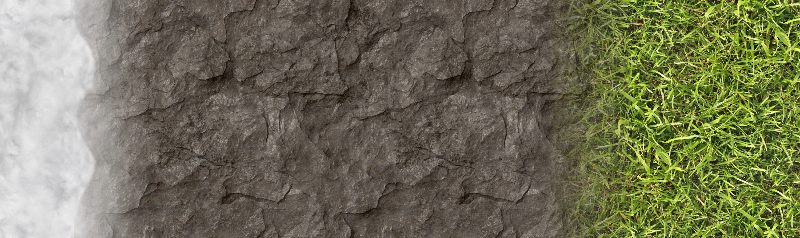
\includegraphics[scale=0.30]{../textures/2DcolorTex.png}
	\caption{colormap 2D}
\end{figure}

\subsubsection{Texture 2D colormap v2}
Voici la version utilisée actuellement de texture colormap :

\begin{figure}[h]
	\center
	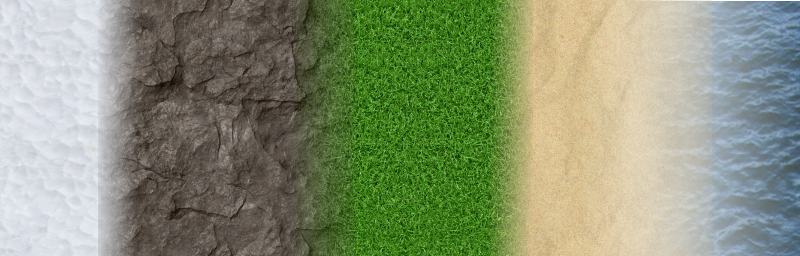
\includegraphics[scale=0.30]{../textures/2DcolorTexv2.png}
	\caption{colormap 2D v2}
\end{figure}

\subsubsection{Textures individuelles}
\begin{minipage}[c]{0.46\linewidth}
\center

\includegraphics[scale=0.2]{../textures/snow.jpg}
\captionof{figure}{Neige}
\end{minipage}\hfill
\begin{minipage}[c]{0.46\linewidth}
\center
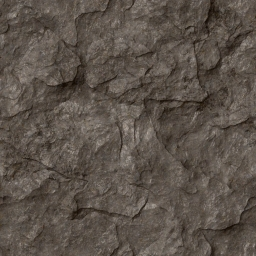
\includegraphics[scale=0.2]{../textures/rock.jpg}
\captionof{figure}{Roche}
\end{minipage}\hfill
\begin{minipage}[c]{0.46\linewidth}
\center
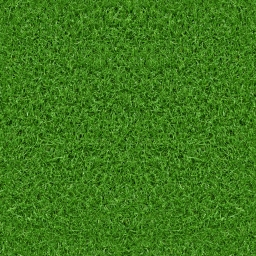
\includegraphics[scale=0.2]{../textures/grass.jpg}
\captionof{figure}{Herbe}
\end{minipage}\hfill
\begin{minipage}[c]{0.46\linewidth}
\center
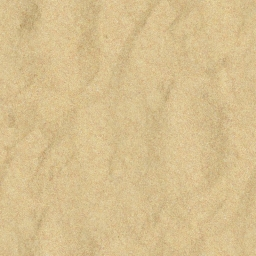
\includegraphics[scale=0.2]{../textures/sand.jpg}
\captionof{figure}{Sable}
\end{minipage}\hfill
\begin{minipage}[c]{0.46\linewidth}
\center
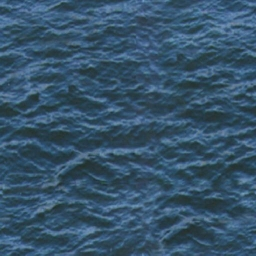
\includegraphics[scale=0.2]{../textures/water.jpg}
\captionof{figure}{Eau}
\end{minipage}\hfill

\section{Problèmes et améliorations}

\subsection{Problèmes}
\subsubsection{Textures}
Nous avons eu un soucis dans un premier temps avec la texture 2D colormap car pour les petites et grandes valeurs de hauteur, la texture "clamp", ce qui n'était visuellement pas très beau.\\

Nous avons remédié au problème en forçant à choisir les textures individuelles pour ces grandes et petites valeurs en les mettant en mode GL\_REPEAT.\\

Il y a également un soucis (toujours présent), pas des plus gênants mais visible tout de même avec le mouvement.

En effet, lorsque l'on avance ou recule, on constate que les textures ont tendance à bouger le long du relief de façon horizontale.\\

Cela s'explique par le fait que nous utilisons les coordonnées du sommet pour accéder aux coordonnées dans la texture.

Or, les coordonnées du sommet changent en fonction du mouvement.

Nous n'avons pas eu le temps de nous pencher sur la question afin de trouver une solution convenable à ce problème.\\

Nous utilisions une texture 1D colormap au départ, et avec celle-ci, nous n'avions bien évidemment pas ces problèmes là.

\subsubsection{Lenteur}

Sur les ordinateurs de l'UFR, nous avons constaté certaines lenteurs avec notre programme.

Sur un ordinateur doté d'une carte graphique Nvidia Geforce GTX 950M, nous n'avons pas vraiment de soucis de lenteur en revanche.

Il se peut qu'il y ait des optimisations à faire pour éviter des gros calculs au GPU.

\subsubsection{Brouillard exponentiel}

Nous avons essayé d'implémenter un brouillard exponentiel qui dépend de la position de la caméra et de la profondeur mais nous n'obtenions pas un résultat convenable.

Nous nous sommes donc rabattu sur un brouillard linéaire.

\subsection{Améliorations}

\subsubsection{Concernant le brouillard}
Il aurait pu être intéressant de créer un brouillard selon la hauteur des sommets (et pas seulement selon la profondeur par rapport à la vue), se rapprochant ainsi des phénomènes de brouillard que l'on constate naturellement sur les hauts sommets.

\subsubsection{Créer des reliefs locaux}
Une autre idée (mais qui aurait pris du temps) aurait été de faire du displacement mapping (au mieux) sur les zones à éventuel relief local comme la roche.

\subsubsection{Paramètres du bruit}
Nous avions pensé à modifier les paramètres du bruit individuellement selon une constante dépendant du vecteur de mouvement, malheureusement nous ne l'avons pas réalisé.
\end{document}